\section{title}
Current collaborative robot solutions guarantee safety, but they use
obstacle detection to stop moving. Our dynamic obstacle avoidance
solution is that of using obstacle detection to respond by moving around the
obstacles while continuing to accomplish the desired tasks. Additionally, our integrated dynamic motion planning approach creates motion
plans that fulfil various task specific constraints for typical industrial
applications. For example the work cell 3D model is used to create a consistent
model of the work environment, so that collision free trajectories are flexibly 
generated for different operations. The automatic consideration of these
constraints  drastically simplifies and speeds-up the deployment of the robot.

An artist's illustration of our dynamic obstacle avoidance solution is shown
in Fig. \ref{fig:overview}. The robot motion control component generates
appropriate motion commands for the robot controller to follow the trajectories required for a given task. The proximity-sensing skin that covers the links and joints of the manipulator, produces information regarding potential collisions. This information is used by the robot motion control
module to adapt the robot motions on the fly to fulfil both constraints:
following the current trajectory (with a certain tolerance) and avoid
collisions. If the collision is unavoidable with local deformations of the
current trajectory, the robot motion control module requests a (global) re-planning,
which is performed on the fly by the reactive path-planner. The motion control
then takes the end effector to the final goal pose using the alternative
trajectory. The main functional modules of the system are discussed in the following
sections of the paper.

\begin{figure}[t]
\centering
\resizebox{0.8\columnwidth}{!}{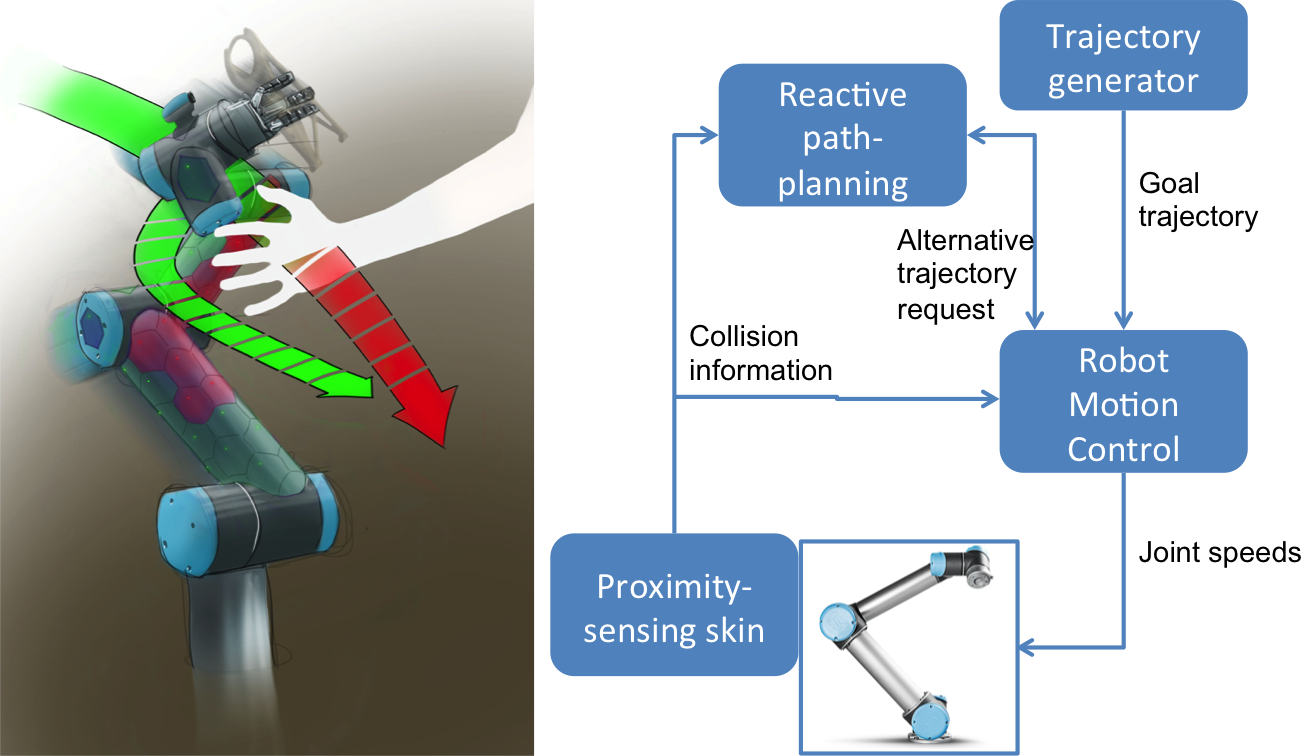
\includegraphics{chapters/doa/images/overview}}
\caption[]{An artist's schematization of the FiaD Dynamic obstacle avoidance
concept is illustrated on the left side. On the right, an overview of the main
components of the solution.}
\label{fig:overview}

\end{figure}

\begin{figure}[h]
\centering
\resizebox{0.8\columnwidth}{!}{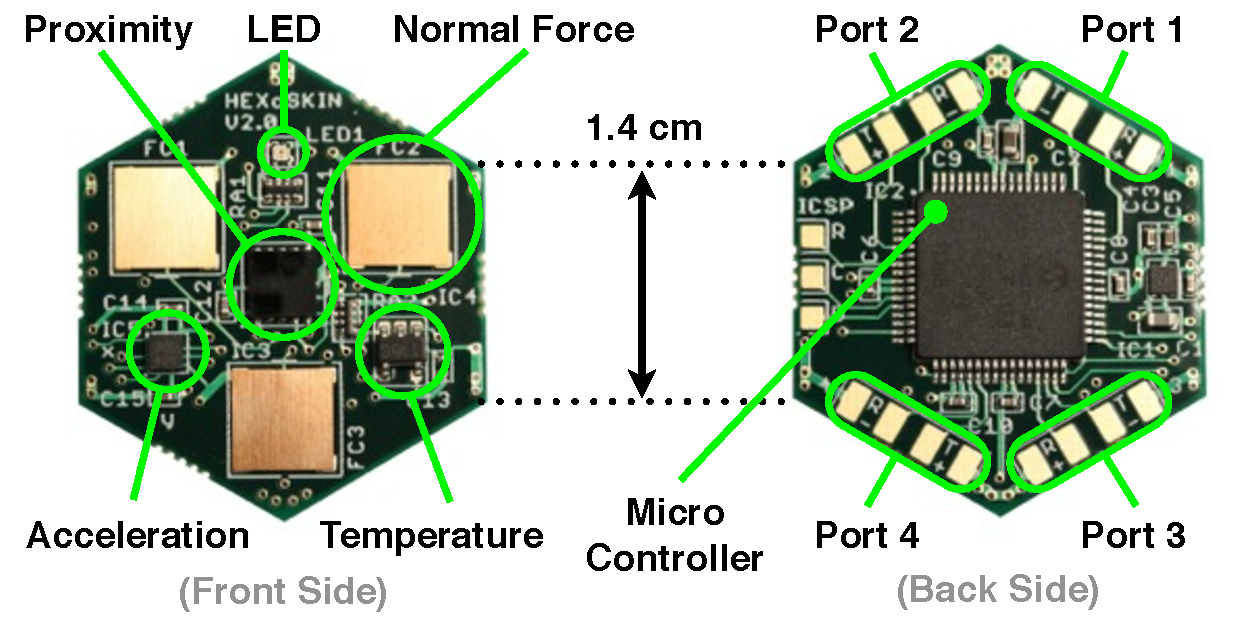
\includegraphics{figures/sensor_unit}}
\caption[]{Robot skin developed at Institute for Cognitive Systems (ICS), TUM.}
\label{fig:RobotSkin}
\vspace{-10pt}
\end{figure}	

Our robot skin system is modularized and transduces multi-modal tactile stimuli \cite{MittendorferYC15}. 
The robot skin consists of hexagonally shaped PCB modules which we call skin cells (see Fig. \ref{fig:RobotSkin}). 
A group of directly connected skin cells is termed skin patch. All skin cells are identical and contain the same set of sensors.
The sensors sample 9 tactile stimuli of 4 different
modalities, namely vibration (3D acceleration sensor), 3 normal forces (capacitive force sensor), 2 temperatures and 1 distance
(optical proximity sensor). These sensors are either off-the-shelf standard ICs or in the case of the force sensors a in-house development.
A microcontroller in the back of each skin cell collects data from its sensors, filters it and creates and sends data packets,
which contain the most recent values of all sensors. All the skin cells are connected to each other via stretchable flex PCBs 
which allows the skin to cover curved surfaces and increases its robustness. The network of skin cells is a meshed bidirectional
communication network which is routed by the microcontrollers of the skin cells. A self-organized algorithm initializes all 
the skin cells in a skin network and constructs a bidirectional communication path between each skin cell and the network root, 
the tactile section unit (TSU). The TSU converts skin network packets to standard UDP Ethernet packets and vice versa.
This allows for fast low latency connections between robot skin and PC (see Fig. \ref{fig:SkinCellNetworkArchitecture}).
\begin{figure}[t]
\centering
\resizebox{0.8\columnwidth}{!}{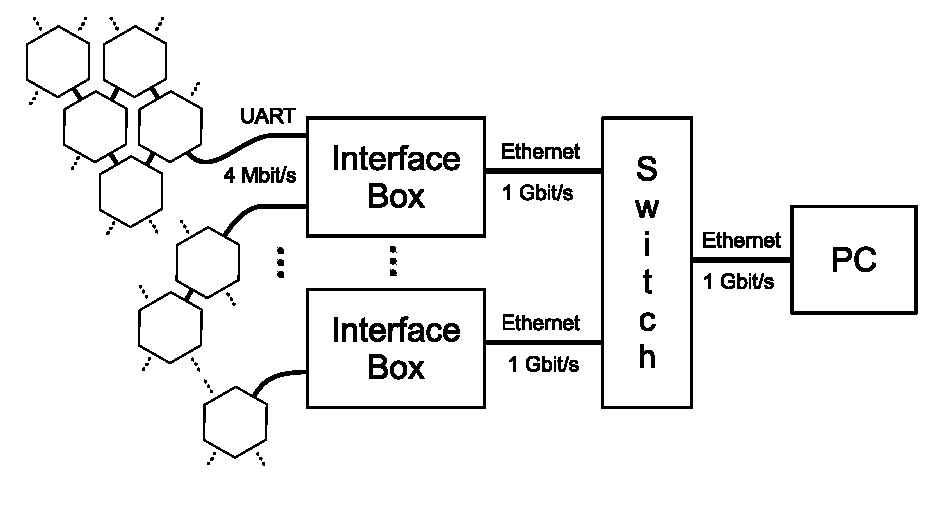
\includegraphics{figures/SkinCellNetwork}}\\[-15pt]
\caption[]{The skin cell network architecture and interface to the PC.}
\label{fig:SkinCellNetworkArchitecture}
\vspace{-10pt}
\end{figure}

The robot skin system also supports the auto-calibration of spatial relationships between skin cells of a skin patch covering a 3D 
surface \cite{Mittendorfer-IROS12tendorfer} such that the kinematic chain of every skin cell to the base frame can easily be determined.  

The proximity sensors used in the skin cells are infrared based sensors. The sensor emits infrared light and captures its reflections on obstacles 
in the range from 0 to 15 cm. The strength of the reflections allows the sensor to estimate the distance between the sensor and detected objects.   

\section{Combining motion Planning and control}
There are three kind of paradigms that classifies robot's architecture\cite{asada1986robot}. The first one being the deliberative architectures work on Sense-Plan-Act strategy with environment models to represent the world. They are less reliable for reactivity and human safety because an erroneous representation of world could result in an unfortunate situation. Reactive architectures work on Sense-Act strategy which encompasses the constraint based local controllers on which we had a short look. Though they are reliable for safety, they are only locally optimal and it is impossible to operate independently. The final architecture and the one we are interested is the hybrid architecture that can combine the potential advantages of both the components to successfully realize complex scenarios without compromising safety and reliability. 

The straight forward way to combine both of them is to execute a trajectory and use reactive techniques to take care of safety. If the robot hits a local minimum or a kinematic/task singularity, re-planning mode could be activated. These reactive techniques should basically deform a planned trajectory to achieve the desired goal while taking care of the safety simultaneously. The hierarchical jacobian controller in fact does trajectory deformations which is granted for free by the solver\cite{escande2014hierarchical}. The proposed method actually exploits the hierarchical nature of the solver to perform the deformations without sacrificing the main goal. 

\section{Reactive Control Framework}
The motion control is achieved using the Stack of Tasks (SoT) controller
framework \cite{Mansard2009} which employs a hierarchical jacobian control strategy eliminating the analytical inverse kinematics computation thus making it a generic controller for all robot platforms. The controller's hierarchical nature allows the robot to handle multiple kinematic tasks simultaneously exploiting the kinematic redundancy of the robot. The controller's real time capability comes from the high computational speed of the state of the art Hierarchical Quadratic Programming (HQP) solver backing it. 


A \emph{task} basically is a control law that achieves a specific objective which can be a free space task or just an inequality constraint that narrows down the workspace of the robot. The task function formalism is very well discussed in \cite{C.Samson1991}. In the context of our work, tasks generally include robot joint posture task, collision avoidance task, joint limits task and so on. The SoT framework handles the task priorities hierarchically in the real time to ensure there are no conflicts among tasks which is used to achieve dynamic obstacle avoidance without compromising on the main goal.

For example, let us consider a pick and place application in a collaborative
environment. The primary goal for this application is to enable a robot to move
to a (set of) desired pick and place locations repetitively. The pick and place
locations can be defined as posture tasks in SoT. However, a higher priority
task considering the collaborative nature of the environment is to avoid
collisions with obstacles that could be humans, for instance. Typically such a
task is modelled as an ``Inequality'' task and an eventual feasible solution (if
one exists) is computed by the solver by exploiting the kinematic redundancy of the robot. In the jargon of motion planning and control, this behaviour is similar to a \emph{local planner}.
However, it is likely that a feasible solution is not found due to the solver
converging to a local minima\footnote{This is caused by the use of task
Jacobians. For further details, please see \cite{Mansard2009}.} In such a
scenario, SoT can also be used to leverage the services of a global planner (see
Section \ref{subsec:reactive_path}) from the current robot state to the goal so
that an entirely new path is obtained which is free from collisions and
consequently allowing all the specified tasks to be achieved in the order of
their priorities. In Section \ref{sec:prelim_results}, we present the
experimental results of using the SoT controller on a practical setup and in
simulation. The SoT controller has also been configured to work with the ROS-control interface. In all these setups, the proximity information from
the artificial robot skin is used as an input to the collision avoidance task. In
the following part, we briefly present the global path planner software framework
that is used when the SoT controller hits a local minima.



\subsection{Stack of Tasks}
'Stack of Tasks' is a hierarchical jacobian-based task controller framework which implements the generalized inverse kinematic formalism by Hanafusa et Al. for local control of redundant systems\cite{hanafusa1981analysis}\cite{Mansard2009ik}. The framework in the earlier stages implemented the Siciliano's extension to handle multiple equality tasks\cite{siciliano1991general}. It has evolved to handle inequality constraints implementing the state of the art solver. The framework provides a structure that orders actives tasks to compute the control law without compromising on the task priority and control continuity. The framework provides a simple scripting interface to interact with controller components during the runtime and has a wrapper to communicate with the ROS world.


\subsection{What is a Task?}
A task basically composes a control law with a specific objective which can be such as reaching a desired joint position, avoiding obstacles in the environment, a visual servoing mechanism for grasping or so on. A task is mainly defined by the error between the desired and current feature, the error jacobian and the gain. These defined tasks are pushed into 'Stack of Tasks' which computes the control law for all the task objectives in an iterative manner\cite{mansard2007task}. 

\[\textit{e(t) = x\textsuperscript{*} - x }\]

where \textit{x} refers to the current state of a feature, \textit{x\textsuperscript{*}} refers to the reference feature.

\subsection{Redundancy Formalism}
Siciliano and Slotine proposed a systematic control framework to compute controller outputs for achieving multiple tasks in redundant systems from the redundancy formalism proposed by Hanafusa et al. The idea is, tasks are solved only in the null space of the higher priority tasks to avoid conflicts with them. This means, a task at any level has no effect on the tasks in the higher level as it uses only the left degrees of freedom. 

Let $(e_{1},J_{1})$ be a primary task  which is defined by  
\begin{equation} \label{eq:tf1}
\dot{e} = J\dot{q} 
\end{equation}
 \textit{J} referring to the Jacobian of the error velocity with respect to joint velocity at the current joint state.


\begin{equation} \label{eq:tf3}
\dot{q} = J_{1}^{+}\dot{e}_{1} + Pz
\end{equation}
 Where \textit{P} is the projector on the null space of the the Jacobian J and \textit{ $z$ } is the arbitrary velocity vector which can be used as a parameter to achieve the secondary objectives. 

Let $(e_{1},J_{1})(e_{2},J_{2})...(e_{n},J_{n})$ be tasks in the stack. The redundancy formalism for two tasks can be extended to n tasks such that $e_{i}$ does not conflict with $e_{j}$ such that $j<i$. 


The recursive joint velocity is of the form
\begin{equation} \label{eq:ntasks}
  \dot{q}_{0} = 0\\
\end{equation}
\begin{equation}
  \dot{q}_{i} = \dot{q}_{i-1}+ (J_{i}P^{A}_{i-1})^{+}(\dot{e}_{i} - J_{i}\dot{q}_{i-1}), i= 1..n
\end{equation}



 where $P^{A}_{i-1}$ is the projector onto the null space of the augmented Jacobian $J_i^A = (J_1...J_i)$ and $\widetilde{J}_i = J_iP_{i-1}^A$ is the limited jacobian of the task. The joint velocity achieving all the task objectives is $\dot{q} = \dot{q}_n$. The recursive projector is computed by 
 
 \[P^A_i = P^A_{i-1} - (J_iP_{i-1}^A)^+J^A_{i-1}  \] 
 
 This systematic way of prioritizing tasks allows simultaneous execution of multiple tasks without conflicting each other.
 
\subsection{Hierarchical Quadratic Programming}
Mansard et al. proposed an improved QP solver to manage multiple equality and inequality problems in a prioritized hierarchy to handle redundancies[15]. The solver handles equality tasks quite the same like in Siciliano's framework but the solver uses complete orthogonal decomposition(COD) instead of Sing for solving the least squares which is quite faster and efficient. The Hierarchical complete orthogonal decomposition(HCOD), a COD of the jacobian mapping for all the levels is used to compute primal optimum for all the constraints at once making it computationally faster. 

Kanoun et al. and De lasa et. al used a primal active search algorithm which is very expensive due to inefficient optimal active set search involving inappropriate activation and deactivation of constraints at each level along the cascade\cite{de2010feature}\cite{kanoun2011kinematic}. The HQP solver depends on a modified primal active search algorithm to make the optimal active set computation much more efficient. Lexicographic optimization formalism is introduced to maintain the active set at each iteration consistent with prior levels completely eliminating unnecessary constraint deactivations and activations. The solver is ten times faster than the classical solvers and can consider inequalities at any levels of the
hierarchy \cite{escande2014hierarchical}.
\subsection{Proximity Distance Gradient for Collision Avoidance}
The computation of the gradient of the proximity distance between the collision bodies inspired from \cite{escandestrictly} is required to define inequality constraints in Stack of Tasks to avoid self-collision and with external obstacles using a proximity sensor. Let $d$ be the distance between approximated collision bodies $O_1(q)$ and $O_2(q)$. The distance between these bodies and its variation is mapped to joint actuations $q$. The distance gradient can be computed by:
\[ \frac{\partial d}{\partial q} = n_d^{'}(\frac{\partial o_1(q)}{\partial q}- \frac{\partial o_2(q)}{\partial q}) \]

where $n_d^{'}$ is the unit normal distance vector while $o_1(q)$ and $o_2(q)$ are the respective closest points. The gradient of the closest point $p$ of fixed coordinates $(\rho_1(q),\rho_2(q)....\rho_l(q))$ in the local reference frame $(e_1(q),e_2(q)...,e_l(q))$ of a collision object at joint configuration $q$ is

\[\frac{\partial p}{\partial q} =  \sum_{l=1}^{d}\rho_l(q)\frac{\partial e_l(q) }{\partial q}\]

In a 3 dimensional workspace, the expression can be written as 

\[ \frac{\partial p}{\partial q} =  (x y  z)J_\omega + J_\nu \]

where $J_\omega$ is the jacobian of the rotational degrees of freedom $J_\nu$ is the jacobian of the linear degrees of freedom. In case of the external objects, the second part of the equation can be eliminated if the object is static. 

\section{KINEO}
\hypersetup{colorlinks, linkcolor=blue}
The reactive path planning software framework is based on the industry grade KineoWorks\texttrademark\footnote{See
\href{http://www.plm.automation.siemens.com/en\_us/products/open/kineo/kineoworks/index.shtml}{Kineoworks}.} path planning library from Siemens in order to provide fast and reliable robot paths. This framework has also been seamlessly integrated into the ROS-ecosystem via a ROS package called \texttt{kws\_ros\_interface} which provides the planner implementations of KineoWorks as shared objects that are readily usable in ROS-based software via the \texttt{kws\_ros\_planner} ROS node.

Robot kinematic models are provided to KineoWorks in the Unified Robot Description Format (URDF) which is a ROS standard. Furthermore, KineoWorks also accepts the standard ROS representation of a \texttt{PointCloud}\footnote{See http://wiki.ros.org/pcl} for creating collision models of dynamic obstacles in the environment. In our work, point clouds are generated in two ways. In one scenario the point clouds are generated by a standard Kinect 3D camera that is observing the immediate environment of the robot. In the other scenario, the point clouds are generated from the proximity data obtained from the Artificial Skin. Finally, the collision detection for dynamic obstacle avoidance is performed using the Kineo\texttrademark Collision Detector (KCD)\footnote{See \href{http://www.plm.automation.siemens.com/en\_us/products/open/kineo/collision-detector/index.shtml}{KCD}.}. KCD performs 3D collision detection and minimal distance analysis between triangular mesh surfaces in assembly environments. KCD has been designed specifically to minimize memory usage and take advantage of parallel processing. The complete software architecture used in our paper for the Dynamic Collision Avoidance functionality is shown in Fig. \ref{fig:dca}.
\begin{figure}[t]
\centering
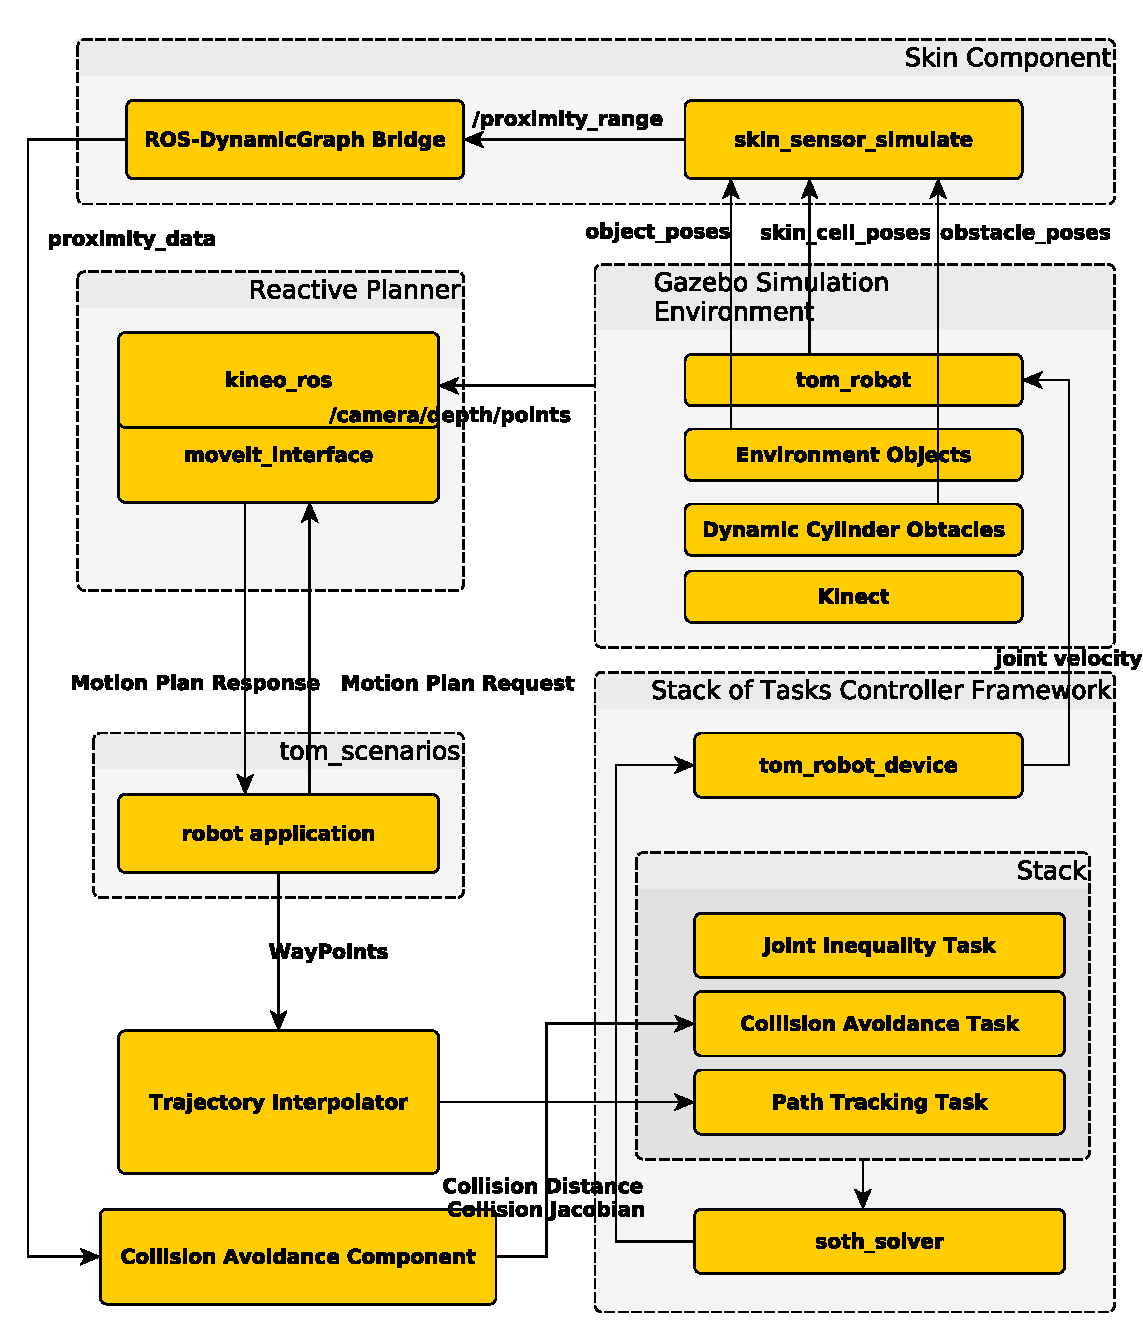
\includegraphics[scale=0.47]{architecture_reactive_collision_1}
% \resizebox{2\columnwidth}{!}{\includegraphics{arch_tom_3}}\\
\caption[]{Dynamic collision avoidance software architecture.}
\label{fig:dca}
\end{figure}

In the following sections we present the current results we have of using the different functionalities described.




\section{Method to combine Path Planning and Reactive Motion Control}
The methodology is based on defining the main goal as a workspace constraint and prioritizing between safety tasks and trajectory execution task (in joint space). The figure \ref{gso} gives an intuitive idea about the stack priority order .
   \begin{figure}[thpb]
      \centering
      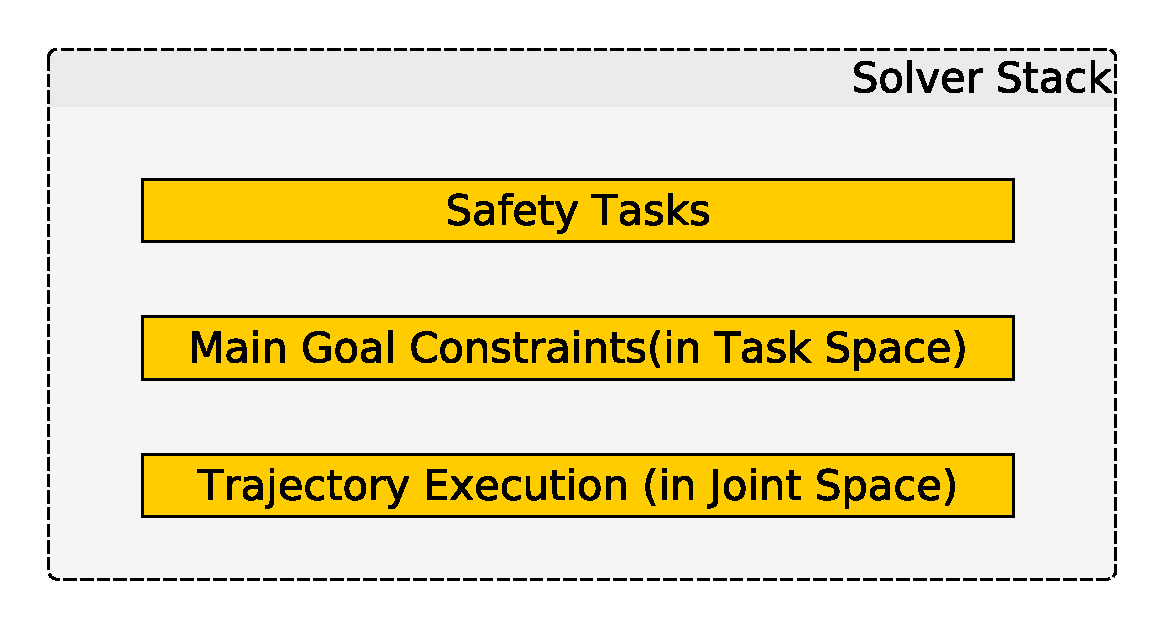
\includegraphics[scale=0.5]{chapters/doa/images/ProposedMethodology.eps}
      \caption{Generic stack order for combining planning and control. The priorities decreases from top to bottom. }
      \label{gso}
   \end{figure}

\begin{itemize}
 \item Safety tasks are obviously given higher priority in the stack for collision avoidance.
 \item Trajectory execution in Joint space occupies the least priority which leaves the controller only the left degrees of freedom from the primary task. If a base trajectory crosses an unforeseen or dynamic obstacle and if the sensors can sense it, the robot basically cannot execute the trajectory until the object is actually moved out of its way. Replanning could be activated if there is no other possibility to reach the joint trajectory goal. Even if there is a possibility to avoid the obstacle and continue executing the  trajectory, it is always not sure that the robot will end up in the desired goal in the task space. 
 
 \item The clever trick here is in the way the main goals are defined. The main goal can be moving a base to a particular pose in the world or move the end effector to a grasping pose. Here the important thing is that the goals are something defined in the workspace though a joint trajectory is executed to achieve them. The hierarchical nature of the controller puts this main goal task in high priority and the jacobian core of the solver finds an optimal solution to follow the main goal. The next section illustrates this methodology on a simple scenario to show the potential of this method.
\end{itemize}
